%%%%%%%%%%%%%%%%%%%%%%%%%%%%%%%%%%%%%%%%%%%%%%%%%%%%%%%%%%
%
% Vzor pro sazbu kvalifikační práce
%
% Západočeská univerzita v Plzni
% Fakulta aplikovaných věd
% Katedra informatiky a výpočetní techniky
%
% Petr Lobaz, lobaz@kiv.zcu.cz, 2016/03/14
%
%%%%%%%%%%%%%%%%%%%%%%%%%%%%%%%%%%%%%%%%%%%%%%%%%%%%%%%%%%



% Možné jazyky práce: czech, english
% Možné typy práce: BP (bakalářská), DP (diplomová)
\documentclass[czech,BP]{thesiskiv}

% Definujte údaje pro vstupní strany
%
% Jméno a příjmení; kvůli textu prohlášení určete, 
% zda jde o mužské, nebo ženské jméno.
\author{Antonín Vrba}
\declarationmale

%alternativa: 
%\declarationfemale

% Název práce
\title{\LARGE Rozpoznávání obličejů pomocí metod založených na lokálních binárních vzorech}

% 
% Texty abstraktů (anglicky, česky)
%
\abstracttexten{
This bachelor thesis deals with testing and enhancing methods which are based on local binary patterns in the face recognition task. The thesis theoretically describes the individual phases of recognition (identification) and the functioning principle of the LBP image descriptor. In addition, based on the LBP there are suggested and implemented two new methods of obtaining binary patterns from the image data. Part of the thesis is an application created for experimental testing of the suggested methods with the use of OpenCV library. For the testing part there was used the new face database ČTK, which contains real photos of actual people. The subject of the experiments is obtaining suitable parameters for high recognition success rate. The experiment results are evaluated and compared to results of other methods in the same face database.}

\abstracttextcz{
Tato bakalářská práce se zabývá testováním a vylepšením metod na bázi lokálních binárních vzorů v úloze rozpoznávání obličejů. Práce teoreticky popisuje jednotlivé fáze procesu rozpoznávání a také princip fungování obrazového deskriptoru LBP. Na základě LBP jsou dále navrženy a implementovány dva nové způsoby získávání binárních vzorů z obrazových dat. Součástí je vytvořená aplikace pro experimentální testování navržených metod s využitím knihovny OpenCV. Pro testování je použita nová obličejová databáze ČTK, která je tvořena reálnými fotografiemi osob. Předmětem experimentů je získání vhodných parametrů pro vysokou rozpoznávací úspěšnost. Výsledky experimentů jsou zhodnoceny a porovnány s výsledkami jiných metod na stejné obličejové databázi.
}

% Na titulní stranu a do textu prohlášení se automaticky vkládá 
% aktuální rok, resp. datum. Můžete je změnit:
%\titlepageyear{2016}
%\declarationdate{1. března 2016}

% Ve zvláštních případech je možné ovlivnit i ostatní texty:
%
%\university{Západočeská univerzita v Plzni}
%\faculty{Fakulta aplikovaných věd}
%\department{Katedra informatiky a výpočetní techniky}
%\subject{Bakalářská práce}
%\titlepagetown{Plzeň}
%\declarationtown{Plzni}

%%%%%%%%%%%%%%%%%%%%%%%%%%%%%%%%%%%%%%%%%%%%%%%%%%%%%%%%%%
%
% DODATEČNÉ BALÍČKY PRO SAZBU
% Jejich užívání či neužívání záleží na libovůli autora 
% práce
%
%%%%%%%%%%%%%%%%%%%%%%%%%%%%%%%%%%%%%%%%%%%%%%%%%%%%%%%%%%

% Zařadit literaturu do obsahu
\usepackage[nottoc,notlot,notlof]{tocbibind}

% Umožňuje vkládání obrázků
\usepackage[pdftex]{graphicx}

% Odkazy v PDF jsou aktivní; navíc se automaticky vkládá
% balíček 'url', který umožňuje např. dělení slov
% uvnitř URL
\usepackage[pdftex]{hyperref}
\hypersetup{colorlinks=true,
  unicode=true,
  linkcolor=black,
  citecolor=black,
  urlcolor=black,
  bookmarksopen=true}

% Při používání citačního stylu csplainnatkiv
% (odvozen z csplainnat, http://repo.or.cz/w/csplainnat.git)
% lze snadno modifikovat vzhled citací v textu
\usepackage[numbers,sort&compress]{natbib}

%%%%%%%%%%%%%%%%%%%%%%%%%%%%%%%%%%%%%%%%%%%%%%%%%%%%%%%%%%
%
% VLASTNÍ TEXT PRÁCE
%
%%%%%%%%%%%%%%%%%%%%%%%%%%%%%%%%%%%%%%%%%%%%%%%%%%%%%%%%%%

\usepackage[toc]{glossaries}

\setlength\parindent{0pt}
\setlength{\parskip}{1em}
 
\usepackage{newfloat}

\DeclareFloatingEnvironment[fileext=lop]{Funkce}
 
\begin{document}
%
\maketitle
\tableofcontents

\chapter{Úvod}

Cílem této práce je seznámit se s nově vzniklou obličejovou databází ČTK a prostudovat metody rozpoznávání obličejů využívající lokální binární vzory. Na základě principu fungování LBP jsou navrženy a implementovány dvě nové metody pro získávání binárních vzorů. S využitím knihovny počítačového vidění OpenCV a programovacího jazyka C\texttt{++} je vyvinuta aplikace pro dlouhodobé testování nově navržených metod. Cílem experimentů je nalezení vhodných parametrů napříč celým procesem rozpoznávání za účelem získání nejlepší možné úspěšnosti. 



Hlavním přínosem této práce by měly být výsledky nově navržených metod rozpoznávání a také způsob nalezení jejich nejvíce vyhovujících parametrů. Jelikož pro obličejovou databázi ČTK existuje zatím jen málo výsledků pro různé druhy rozpoznávacích algoritmů, je možné tuto práci považovat za přínos i v této oblasti.
 
\chapter{Teoretická část}

\section{Rozpoznávání obličejů}
Identitu člověka lze určit na základě různých biometrických faktorů. Existuje mnoho používaných metod jakými jsou například: otisk prstu, oční sítnice nebo dynamika chůze. Jedním z nejžádanějších způsobů identifikace poslední doby je rozpoznávání osob podle jejich obličeje. Snažíme se počítače naučit rozpoznávat obličeje stejně dobře nebo i lépe než dokážeme my rozpoznávat osoby z našeho  okolí. V posledních letech se také tato disciplína stala velmi atraktivní i pro výrobce kamerových a bezpečnostních systémů. S nárůstem výpočetního výkonu a razantním zlepšením kvality záznamu se na trhu objevují první \uv{smart} bezpečnostní systémy s podporou rozpoznávání osob. Avšak i po 45 letech výzkumu v této oblasti máme v obtížných podmínkách stále rezervy. Je zde tedy prostor pro další výzkum a nalézání nových metod rozpoznávání.

\subsection{Detekce obličeje}
Počátečním problémem k cestě za úspěšným stanovením identity je nalezení obličeje ve vstupních obrazových datech. Často užívanou metodou pro detekci libovolných objektů je metoda Haarových kaskád známá též jako Viola-Jones algoritmus, který byl představen v roce 2001 \citet{ViolaJones2001}. Princip metody spočívá v natrénování klasifikátoru, který v trénovacích datech (obličejích) nachází Haarovy vzory - primitiva reprezentující sumu jasových složek pod ním viz Obrázek \ref{fig:haar}. Tyto primitiva a jejich pozice se nacházejí uvnitř trénovacího rámce o velikosti např. $24\times24$px. Tento rámec se poté posouvá po vstupním obraze a testuje se umístění sady naučených primitiv. Vstupní obraz se může předzpracovat na tzv. integrální tvar, který obsahuje v pravidelných bodech informaci o lokálním součtu hodnot pixelů. Vzory lze aplikovat na určenou oblast v kaskádách podle jejich významu, nejdříve jsou tedy testovány velká primita a až po jejich úspěšném nalezení potenciálního obličeje je použita další sada primitiv, která může případně úspěšnou detekci více zpřesnit nebo vyvrátit. Při použití pouhých 200 vzorů byla na frontální obličejová data naměřena úspěšnost $95\%$. Pro obrázek s rozlišením $384\times 288$px trvala detekce $0.7$ sekundy. 

Práce z roku 2011 \citet{Herta2011} poukazuje na výpočetní náročnost obličejové detekce v reálném čase a také je pro nás ukazatelem desetiletého pokroku od uvedení algoritmu \cite{ViolaJones2001}. Byl zpracováván video stream s rozlišením $1920\times1080$px při 25 snímcích za sekundu, datový tok činil $3520Kbs$. Implementovaný systém dokázal analyzovat kontinuálně každý snímek videa na který byl aplikován obličejový detektor na bázi Haarových kaskád s časem výpočtu menším než 40ms. Paralelní výpočty prováděla grafická karta s podporou technologie CUDA\footnote{Architektura pro spouštění programů v C/C\texttt{++} na grafickém HW.}.

\begin{figure}[h!]
\begin{center}
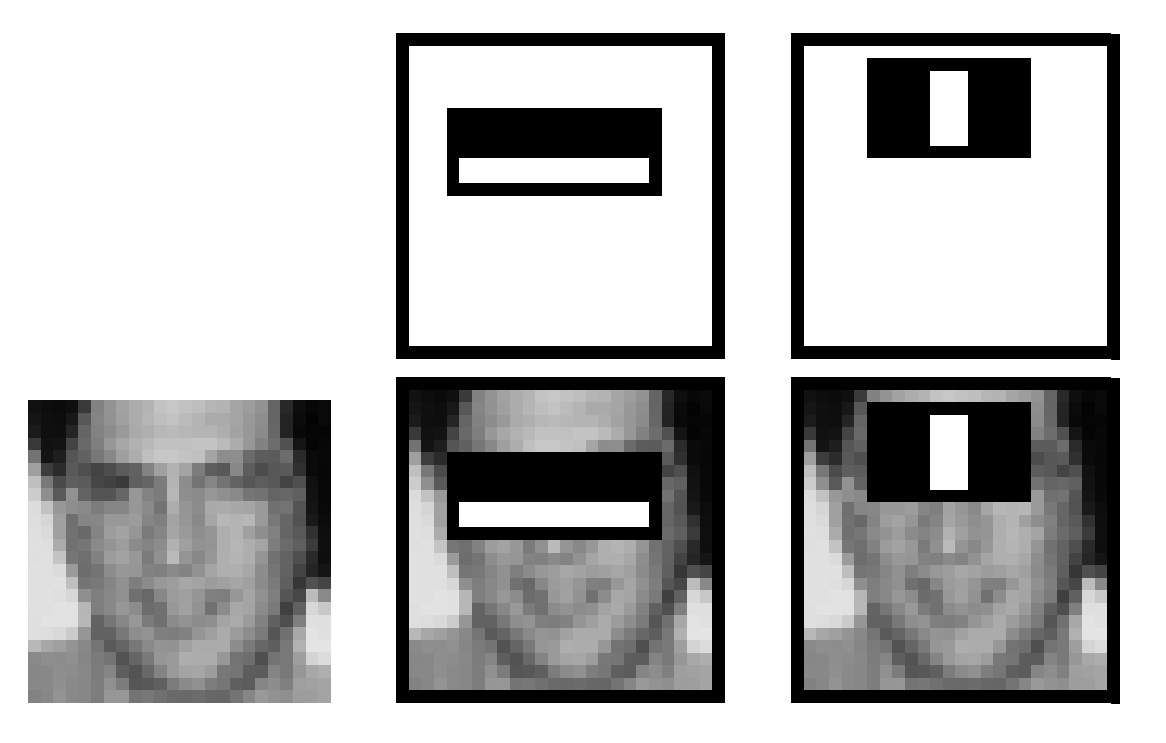
\includegraphics[width=230px]{img/haar_face.png}
\caption{Základní vzory reprezentující rozdílný odstín očí proti tvářím nebo nosu. Převzato z \cite{ViolaJones2001}.}
\label{fig:haar}
\end{center}
\end{figure}

\subsection{Proces rozpoznávání}
Rozpoznávání obličeje je proces, který na základě vstupních dat určí identitu hledané osoby. Určení identity může a nemusí být správné. Úpravou jednotlivých funkčních částí procesu a opakováním experimentu usilujeme o nejvyšší možnou správnost výsledku. V následujícím výpisu jsou popsány funkční celky procesu:
 
\begin{enumerate}
\item Načtení vstupních dat z databáze obličejů
\item \textbf{Předzpracování obrazu} Obličej je detekován, provede se normalizace a oříznutí. Často se obrázek převadí na jednokanálový barevný model (šedotónový).
\item \textbf{Extrakce příznaků} Z obrazu je extrahován příznakový vektor pomocí zvoleného deskriptoru.
\item \textbf{Klasifikace} Testovaným obličejům je přiřazena identita zvoleným klasifikátorem.
\item Vyhodnocení úspěšnosti
\end{enumerate}

Tučně vyznačené sekce mají kritický vliv na úspěšnost celého procesu. Po vyhodnocení se obvykle upraví parametry kritických sekcí a proces se opakuje. Opakování experimentu lze při vhodné implementaci provádět bez potřeby znovunačtení dat. 

\section{Databáze obličejů}
Pro testování a ladění metod rozpoznávání obličejů vzniklo v průběhu let několik databází. Součástí databáze jsou trénovací a testovací data. K jedné testované osobě se většinou váže více než jeden obrázek z dat trénovacích. Obličejové sady se liší obtížností i svým rozsahem. V práci \citet{LencUfi2015} jsou uvedeny známé a stále používané databáze:

\begin{itemize}
\item \textbf{AT\&T} Databáze též známá jako databáze ORL. Obrázky byly pořízeny během let 1992 až 1994. Obsahuje snímky 40 lidí, 10 pro každou osobu s černým pozadím. Fotografie zachycují různá natočení a výrazy v obličeji. Rozlišení obrázků je $92\times 112$px.
\item \textbf{FERET} Obsahuje $14\,051$ snímků $1\,199$ osob pořízených během let 1993 až 1996 v rozlišení $256\times 384$px. Snímky jsou dále rozděleny do jednotlivých kategorií podle natočení obličeje a podle této vlastnosti se dále rozdělují na jednotlivé testovací skupiny. Použití rozpoznávacích algoritmů na všechny testovací skupiny poté v úspěšnosti odráží i schopnost rozpoznávání natočených obličejů.
\item \textbf{AR} Čítá více než $4\,000$ barevných snímků 126 osob z roku 1998. Rozlišení snímků je $768\times 576$px. Fotografie jsou pořízeny v různých světelných podmínkách a s různým výrazem v obličeji. Jsou zde zastoupeny i osoby s brýlemi nebo se zahalenými částmi obličeje. 
\end{itemize}

\subsection{Nová databáze obličejů ČTK}
Práce \citet{LencUfi2015} představuje nově vzniklou obličejovou databázi (2015). Je tvořena reálnými fotografiemi z fotoarchivu ČTK\footnote{Česká Tisková Kancelář}. Databáze má dvě části:

\begin{enumerate}
\item Unconstrained Facial Images (UFI) - Obsahuje obrázky 530 osob o velikosti $384\times384$px. Každá osoba vlastní v průměru $8.2$ fotografií. Obličeje jsou na libovolných místech fotografie viz Obrázek \ref{fig:ufi1} v proměnlivých velikostech. Pro zpracování takové databáze je nejdříve nutné obličeje detekovat a vhodně obrázky předzpracovat. 
\item Cropped images - Obsahuje fotografie 605 osob v rozlišení $128\times128$px. Každá osoba vlastní v trénovací sadě průměrně $7.1$ fotografií. Tvorba této sady zahrnovala detekování obličeje Viola-Jones algoritmem a nalezení pozice očí. Předzpracování spočívalo v rotaci obličeje podle horizontální linie očí a následné škálování na požadovanou velikost $128\times 128$px viz Obrázek \ref{fig:cropped1}. Používání této sady dat nevyžaduje vlastní implementaci předzpracování, které by výrazně ovlivnilo výslednou úspěšnost.
\end{enumerate}

\begin{figure}[h!]
\centering
\begin{minipage}{.4\textwidth}
  \centering
  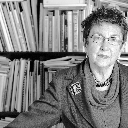
\includegraphics[width=0.7\linewidth]{img/ufi1.png}
	\caption{Ukázka UFI obrázku. Převzatu z \cite{Ufi2015online}.}
  \label{fig:ufi1}
\end{minipage}%
\hspace{1.5cm}
\begin{minipage}{.4\textwidth}
  \centering
  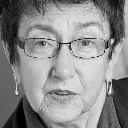
\includegraphics[width=.7\linewidth]{img/cropped1.png}
  \caption{Cropped obrázek. Převzato z \cite{Ufi2015online}.}
\label{fig:cropped1}
\end{minipage}
\end{figure}

ČTK databáze je označena jako obtížná a to díky reálným fotografiím nižší kvality. Článek \cite{LencKral2016} srovnává výsledky základních a rozšířených rozpoznávacích metod na databázích: AT\&T, FERET, AR a ČTK. Výsledky podle neupravené \uv{baseline} verze algoritmu \cite{Ahonen2004} z roku 2004 jsou v pořadí vyjmenovaných databází: $56.17\%$, $93.89\%$, $87.71\%$, $39.81\%$. Zde je vidět markantní rozdíl úspěšnosti na nově vytvořené databázi proti stávajícím. Databáze se tak stává velkou výzvou pro nově vzniklé metody rozpoznávání.

\section{Lokální Binární vzory}
Originální LBP\footnote{Local Binary Patterns (Lokální Binární Vzory)} operátor byl představen v roce 1996 jako velice schopný obrazový deskriptor. Operátor popisuje jednotlivé pixely obrazu pomocí porovnání sousedních pixelů $3\times3$ a centrálního pixelu. Každý pixel je popsán binárním číslem a utváří histogram četností, který lze považovat za deskriptor reprezentující daný obraz. \citet{Ahonen2004} 

Funkce \ref{fig:function1} akceptující parametry $n$ a $c$ reprezentují hodnoty sousedního a centrálního pixelu.  

\begin{equation} \label{fig:function1}
f(n,c) = \begin{cases}
    1  & \quad n \geq c\\
    0  & \quad n < c\\
  \end{cases}
\end{equation}

Na Obrázku \ref{fig:lbp_basic} je znázorněný výpočet binární hodnoty popisující centrální pixel. Významnou výhodou LBP operátoru je invariace vůči světelné intenzitě. Pokud rovnoměrně osvítíme zkoumanou strukturu, výsledné LBP vzory budou mít stejnou hodnotu. Další výhodou je velice jednoduchý výpočet a je velice jednoduché jej modifikovat. Podle binární sekvence kolem středového pixelu lze určit, zda se středový pixel nachází u hrany tmavšího a světlejšího přechodu, této skutečnosti se může dále využít viz podsekce \ref{uniform_lbp}.

\begin{figure}[h!]
\begin{center}
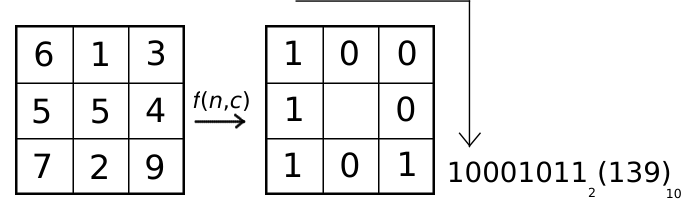
\includegraphics[width=250px]{img/LBP_basic.png}
\caption{Základní LBP operátor}
\label{fig:lbp_basic}
\end{center}
\end{figure}

\subsection{Obecné LBP}
Základní LBP operátor lze zobecnit přidáním dvou parametrů $(P,R)$. Kde $P$ označuje počet bodů a $R$ poloměr kružnice na které se body nacházejí. Operátor poté označujeme jako $LBP_{P,R}$ viz Obrázek \ref{fig:lbp_circular}. Před aplikací operátoru se provádí interpolace bodů na kružnici do tabulky pozic, která se poté používá pro výběry hodnot pixelů na konkrétní pozici.

\begin{figure}[h!]
\begin{center}
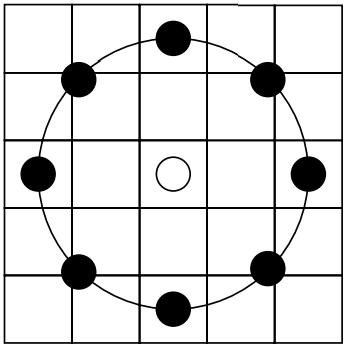
\includegraphics[width=70px]{img/circular_lbp.png}
\caption{Obecný $LBP_{8,2}$ operátor. Převzato z \cite{Ahonen2004}}
\label{fig:lbp_circular}
\end{center}
\end{figure}

\subsection{Uniformní rozšíření LBP} \label{uniform_lbp}
Číslo \textit{P} udává počet sousedních pixelů v okolí \textit{R}. Potom histogram četností, kdy $P=8$ čísel musí nutně mít $2^P$ pozic. Můžeme však tento počet výrazně zmenšit a uvažovat jen taková $8$-bitová čísla, která mají žádný nebo maximálně $2$ přechody z hodnoty $0$ na $1$ a obráceně, pokud se na číslo díváme jako na cyklický buffer. Příkladem takových uniformních čísel jsou: $00000000$, $11110000$, $10000001$. Víme, že taková čísla reprezentují podstatné informace z obrázku (hrany, rohy, linie nebo neměnnou plochu). Histogram lze díky této vlastnosti zmenšit na pouhých 58 pozic, vzory které nesplňují uniformní podmínky jsou umístěny na přidanou pozici 59. Počet uniformních vzorů lze vypočítat pomocí vzorce $P(P-1)+2$. Pro $16$ sousedních pixelů je tedy redukován počet binů\footnote{určitý interval histogramu} z 65536 na 242, což představuje obrovskou paměťovou úsporu za cenu malé ztráty obrazových dat viz Obrázek \ref{fig:uniform_non_uniform} na kterém jsou vykresleny pouze pixely pro které byla hodnota uniformní nebo neuniformní. Při použití uniformních vzorů se používá označení $LBP_{P,R}^{u2}$.

\citet{Ahonen2004} Experimenty s texturami ukázaly, že $90\%$ vzorů je uniformních při použití základního LBP operátoru $LBP_{8,1}$ a okolo $70\%$ při $LBP_{16,2}$.

\begin{figure}[h!]
\begin{center}
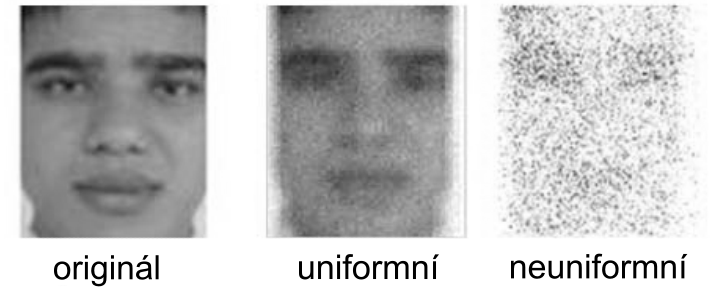
\includegraphics[width=210px]{img/uniform_non_uniform.png}
\caption{Vykreslení pouze uniformních a neuniformních pixelů. Převzato z \cite{Rahim2013}.}
\label{fig:uniform_non_uniform}
\end{center}
\end{figure}

\subsection{Histogram jako příznakový vektor} \label{section_histograms}
Po výpočtu LBP vzorů pro celý obrázek lze vytvořit histogram četností výsledných vzorů. Tento přístup lze použít při popisu jednolité struktury, ale pro obličejová data není vhodný. Obličej nás zajímá z pohledu prostorového rozložení různých elementů, které dokážeme popsat lokálními četnostmi vzorů. Rozložením obličeje na vhodný počet podhistogramů libovolné velikosti lze dosáhnout dobrého popisu obličeje. Složení podhistogramů za sebe poté utváří příznakový vektor. Práce \citet{Vojta2015} se zabývá srovnáním různých obrazových deskriptorů. Z výsledků lze usoudit, že lze najít optimální velikost pravidelné $n\times n$ mřížky podhistogramů.

Zpřesnění popisu obličejových dat je dále možné pomocí váhování jednotlivých podhistogramů. Důležité oblasti na obrázku lze přiřadit různou váhu např. oblast očí, úst atd. V práci \cite{Vojta2015} se díky genetickému algoritmu podařilo nalézt masky vah, které dokáží zvýšit úspěšnost rozpoznávání až o $9\%$. V práci \cite{Lopez2010} je představena maska, která upřednostňuje obličejové prvky a vynechává oblasti s malou informační hodnotou viz Obrázek \ref{fig:weighted}. Přiřazení vah koresponduje s Obrázkem \ref{fig:7x7lbp82}.
 
\begin{figure}[h!]
\centering
\begin{minipage}{.4\textwidth}
  \centering
  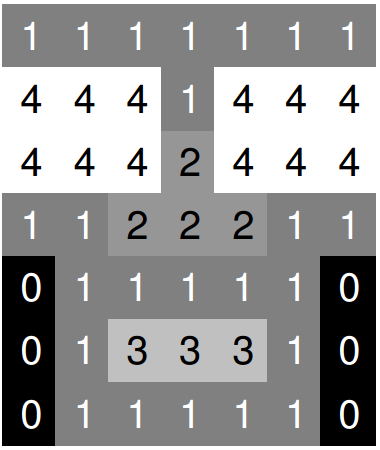
\includegraphics[width=0.39\linewidth]{img/histogram_weights.png}
	\caption{Váhy pro jednotlivé podhistogramy. Převzatu z \cite{Lopez2010}.}
  \label{fig:weighted}
\end{minipage}%
\hspace{1.5cm}
\begin{minipage}{.4\textwidth}
  \centering
  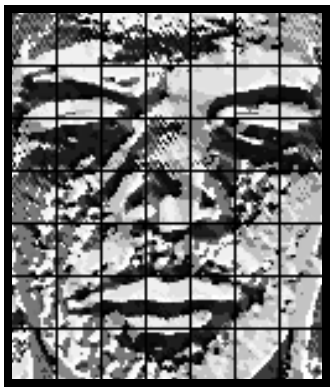
\includegraphics[width=.4\linewidth]{img/subhistograms.png}
  \caption{Mřížka podhistogramů $7\times 7$ na obličeji po aplikaci $LBP_{8,2}^{u2}$. Převzato z \cite{Lopez2010}.}
\label{fig:7x7lbp82}
\end{minipage}
\end{figure}

\subsection{Gáborovy filtry}
Práce \citet{LencKral2016} se zabývá rozšířením LBP operátoru nahrazením pravidelné podhistogramové mřížky soustavou úmyslně pozicovaných podhistogramů. Podhistogramy jsou umisťovány na \uv{zajímavá} místa v obrázku na základě aplikace Gáborových filtrů. Gáborovy filtry se používají v obrazové analýze díky své schopnosti zachytit důležité informace např. detekovat hrany v obrázku tím nám mogou po vhodném nastavení parametrů zvýraznit oblasti obličeje jako jsou oči, ústa nebo nos. Parametry se skládají z vlnové délky, orientace, poměru stran a propustnosti. Na Obrázku \ref{fig:gabor} jsou v horní části vizualizovány samotné Gáborovy funkce a poté i jejich aplikace na obrázek obličeje. 

\begin{figure}[h!]
\begin{center}
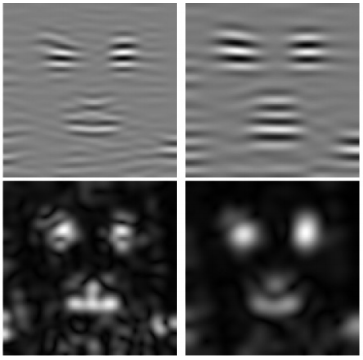
\includegraphics[width=100px]{img/gabor.png}
\caption{Příklady obrázku filtrované pomocí Gáborových filtrů. Převzato z \cite{LencKral2016}.}
\label{fig:gabor}
\end{center}
\end{figure}

Nalezení výchozích bodů pro výpočet podhistogramů lze provést metodou klastrování. Po výpočtu Gáborových filtrů je provedeno prahování výsledného obrazu a na pozice bodů s vysokou intenzitou je aplikována klastrovací metoda K-means, která redukuje počet těchto bodů na požadovanou hodnotu viz Obrázek \ref{fig:gabor_points}. Jelikož jsou Gáborovy filtry náročné na výpočet lze pro všechny obličeje vytvořit globální masku výchozích bodů na základě náhodně vybraného vzorků z trénovacích dat. Z výsledků práce \cite{LencKral2016} je vidět signifikantní nárůst úspěšnosti při experimentech na obličejové databázi ČTK kde bylo dosáhnuto o $20\%$ více úspěšnosti než klasická metoda LBP s pravidelnou mřížkou podhistogramů.

\begin{figure}[h!]
\begin{center}
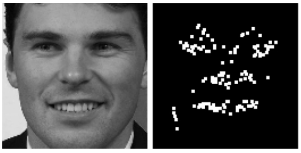
\includegraphics[width=110px]{img/gabor_points.png}
\caption{Originální obrázek a jeho výchozí body (64 klasterů). Převzato z \cite{LencKral2016}.}
\label{fig:gabor_points}
\end{center}
\end{figure}

\section{Porovnání obličejů}
Uvážíme-li metodu pro extrahování příznaků $LBP_{8,1}^{u2}$ a pravidelnou mřížku podhistogramů o rozměru $10\times 10$, výsledný příznakový vektor bude mít $100 \times 59$ položek. Vzdálenost mezi příznakovými vektory určujeme součtem vzdáleností jejich jednotlivých podhistogramů. Máme-li příznakový vektor $A$ můžeme k hodnotám podhistogramů přistoupit stejně jako do dvourozměrného pole $A[i][j]$, kdy $i$ označuje index podhistogramu a $j$ index jeho hodnoty.  

Jednou z nejznámějších metod k určení vzdálenosti v $n$-rozměrném prostoru je Euklidovská vzdálenost $(d)$, která je dána vztahem:

\begin{equation} \label{fig:euclidean}
d(A,B)=\sum_{i=0}^{n}{\sqrt{
\sum_{j=0}^{k}{(
A[i][j]-B[i][j])^2}}}
\end{equation}

Intersekce histogramů $(HI)$ se používala při vyhledávání podobných obrázků v databázích (image retrieval) je dána předpisem:

\begin{equation} \label{fig:histogram_intersection}
HI(A,B)=\sum_{i=0}^{n}{\Bigg[
\sum_{j=0}^{k}{A[i][j]}
-
\sum_{j=0}^{k}{
min(A[i][j],B[i][j])}
\Bigg]
}
\end{equation}

\subsection{Klasifikace}

Běžně používaným algoritmem pro klasifikaci je Nearest-Neighbor\footnote{1NN - nejbližší soused} klasifikátor. 1NN klasifikace obličeje spočívá v  porovnání a nalezení minima vzdálenosti se všemi obličeji v databázi. Pokud databáze obsahuje více záznamů hledaného obličeje, lze klasifikátor upravit na $K$-Nearest-Neighbor, přiřazení identity se následně vyhodnocuje z $N$ nejbližších výsledků a je přiřazena třída (identita) s nejvyšší četností. Na konci procesu rozpoznávání se provede validace výsledků a výstupem je číslo $p$ reprezentující úspěšnost rozpoznáváníviz vztah \ref{fig:accuracy}, kde $c$ je počet dobře identifikovaných osob a $b$ počet chybných.

\begin{equation} \label{fig:accuracy}
p=\dfrac{c}{c+b}\quad p \in [0,1]
\end{equation}

\section{Další obrazové deskriptory}
Dobrá reprezentace objektu, v našem případě obraz obličeje je klíčová pro dobrý systém rozpoznávání. Setkáváme se s problémy, které části obrazu jsou podstatné pro danou úlohu a jak je správně extrahovat. Efektivní deskriptor by měl spolehlivě reprezentovat svůj zdrojový obraz, aby bylo co nejsnadnější určit do jaké třídy patří. Dobrý deskriptor si lze představit tak, že v \textit{n}-rozměrném prostoru bude obličeje dvou a více osob separovat do vlastních shluků (tříd). Mělo by docházet k co nejméně interakcemi mezi třídami. Výhodou deskriptoru je také jednoduchost jeho výpočtu. Jedna z prvních metod, která se ukázala v tomto smyslu jako úspěšná se nazývá Eigenfaces a byla představena již v roce 1991 viz sekce \ref{eigenface}. O několik let později byla představena metoda LBP a překonáním všech dříve známých metod v oblasti rozpoznávání obličejů ukázala směr dalšího vývoje deskriptorů. V článku \citet{Zhang2010} z roku 2010 je kromě výčtu dříve používaných deskriptorů představen nový deskriptor LDP. Ve stejném roce byl také představen pokročilý deskriptor POEM v práci \citet{Alice2010} viz sekce \ref{poem} jenž dosahuje lepších výsledků než LBP i LDP \cite{Vojta2015}.

\subsection{Eigenfaces} \label{eigenface}
V práci \citet{Turk1991} byla poprvé představena metoda Eigenfaces. Vstupní obličejová sada má velikost $N$ obličejů. Pro každý obličej s velikostí $K\times K$ pixelů je vytvořen vektor o $K^2$ dimenzích a obsahuje všechny hodnoty z obrázku (po řádkách). Tyto vektory jsou umístěny do matice o rozměru $K^2\times N$, kde každý obličej reprezentuje jeden sloupec matice. Na tuto matici je aplikována metoda zvaná PCA (Principal Component Analysis), analýzou hlavních komponent matice je redukován její rozměr na požadované \textit{m} tedy $K^2\times m$ tzv eigen-vektory viz Obrázek \ref{fig:eigen_vectors}. Převedeme-li zpět sloupce na obrazová data, dostáváme sadu obrazů reprezentující změny proti průměrnému obličeji ze vstupních dat. Každý nový obličej poté vyjádříme (projektujeme) jako součet průměrného obličeje a lineární kombinace eigen-vektorů. Z kombinace eigen-vektorů a jejich zastoupením v reprezentaci neznámého obrazu lze získat procentuální vyjádření o podobnosti k osobě ze vstupních (trénovacích) dat. Velkou nevýhodou této metody je citlivost na změnu světelných podmínek a přidání obličeje do naučených eigen-vektorů vyžaduje opětovné přepočítání celé matice.

\begin{figure}[h!]
\begin{center}
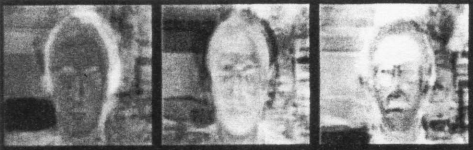
\includegraphics[width=230px]{img/eigen_vectors.png}
\caption{Převedení eigen-vektorů zpátky do obrazové podoby. Převzato z \cite{Turk1991}.}
\label{fig:eigen_vectors}
\end{center}
\end{figure}

\subsection{POEM} \label{poem}
Tento deskriptor s názvem Patterns of Oriented Edge Magnitudes je schopný získat bohaté informace o vstupním obrazu. V práci \cite{Alice2010} je popsán způsob výpočtu deskriptoru a také výsledky experimentů. Obraz je nejdříve převeden na gradientní podobu a každý pixel reprezentuje 2D vektor, jehož velikost odpovídá intenzitě pixelu v gradientním obraze. Dále je obraz diskretizován do podoby, kdy uvažujeme jen určitý počet $p$ dovolených směrů vypočítaných vektorů viz \ref{fig:poem_calculation}. Pro každý pixel je přiřazen vektor reprezentující lokální histogram, který má $p$ položek (binů) a obsahuje četnosti směru okolních vektorů, toto okolí se nazývá \uv{cell}. Hodnoty jsou dále zakódovány pomocí již známé metody $LBP_{P,R}^{u2}$, kde \textit{R} označuje poloměr oblasti známé též jako \uv{block} a uloženy do dílčích histogramů viz sekce \ref{section_histograms}. Pro každý pixel není zakódována jen lokální hodnota popisující tvar nebo přechod jako je tomu při použití samnotného LBP deskriptoru, ale je zde také vztah informací mezi okolními regiony v obrázku. Díky této schopnosti se dokáže POEM velice dobře vyrovnat s natočením obličejům, změnám osvětlení a různým výrazům v obličeji. Z experimentů \cite{Alice2010} je patrné, že pro 3 diskretizační směry je vhodná velikost $7\times 7$px pro \uv{cell} a $10\times 10$px pro \uv{block}, na obličejové databázi FERET bylo tímto deskriptorem dosaženo až o $45\%$ lepších výsledků proti použití klasické metodě LBP.

\begin{figure}[h!]
\begin{center}
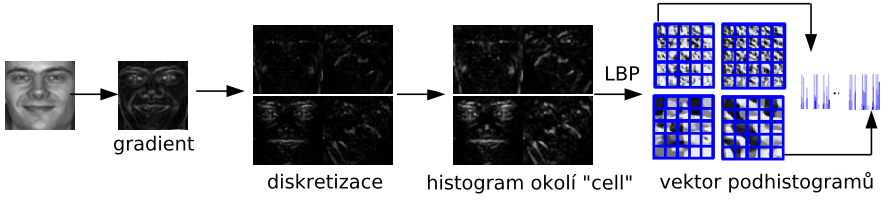
\includegraphics[width=340px]{img/poem.png}
\caption{Výpočet POEM deskriptoru. Převzato z \cite{Alice2010}.}
\label{fig:poem_calculation}
\end{center}
\end{figure}

\section{Knihovna OpenCV}
Celým názvem Open Source Computer Vision Library je volně dostupná knihovna určená pro úlohy počítačového vidění psaná nativně v jazyce C\texttt{++}. Obsahuje stovky optimalizovaných algoritmů a datových struktur pro práci s obrazovými daty. Algoritmy mají uplatnění v detekci a rozpoznávání oblečejů, sledování objektů, identifikace osob, sledování pohybu očí a dokonce pro práci s virtuální realitou. Knihovna je neustále vyvíjena, poslední verze $3.2$ je dostupná na všechny větší platformy: Windows, Linux, Mac, Android a IOS. Rozhraní přes které lze knihovnu používat podporuje programovací jazyky: C\texttt{++}, C, Python, Java a MATLAB. \cite{OpenCV2016online}

OpenCV má modulární strukturu složenou ze sdílených\footnote{ *.so soubory (Linux) pro referencování kódu za běhu programů} a statických\footnote{ *.a soubory (Linux) přímo linkované do programu během kompilace} knihoven \cite{OpenCVmanual2016}. Pro rozpoznávání obličeje jsou užitečné následující moduly: 

\begin{itemize}
\item \textbf{Core funcionality} - datové struktury, vícerozměrná pole cv::Mat, základní funkcionalita pro ostatní moduly 
\item \textbf{Image processing} - lineární a nelineární filtry, transformace obrazu, převody barevných modelů, histogramy
\item \textbf{video} - analýza videa, sledování objektů
\item \textbf{features2d} - deskriptory a hledání jejich společných vlastností
\item \textbf{objdetect} - detekce objektů (obličeje, oči, osoby, auta \ldots)
\item \textbf{highgui} - základní prvky grafického uživatelské rozhraní (okna, posuvníky \ldots)
\item \textbf{Video I/O} - záznam videa a kodeky
\item \textbf{gpu} - akcelerace výpočtů přes grafický HW (CUDA, OpenCL\footnote{paralelní programování heterogenních počítačových systémů})
\end{itemize}

OpenCV se díky své velké komunitě a podrobné dokumentaci stává nejčastější volbou pro experimentální i komerční vývoj aplikací v oblasti počítačového vidění již od roku 1999 kdy byla uvolněna první alpha verze.

\clearpage

 
% 
% PRO ANGLICKOU SAZBU JE NUTNÉ ZMĚNIT
% CITAČNÍ STYL!
%
\bibliographystyle{csplainnatkiv}
{\raggedright\small
\bibliography{literatura}
}


\end{document}
